%!TEX root = ../slides.tex
\section{Методы сегментации ПЭТ изображений}
\begin{frame}
    \frametitle{Методы сегментации ПЭТ изображений. Общая информация}
    \begin{itemize}
        \item Без ограничения общности, сегментацию изображений
        можно представлять как две связанные задачи:
        \textit{распознавание} и \textit{оконтуривание}.
        \item Внешние и внутренние факторы, значительно
         влияющие на сегментацию ПЭТ-изображений:
         \begin{itemize}
             \item проблемы, связанные с разрешением изображения
             \item многовариантность форм, текстуры и расположения патологий
             \item шум
         \end{itemize}
        
    \end{itemize}
\end{frame}

\begin{frame}
    \frametitle{Методы}
    \begin{figure}
        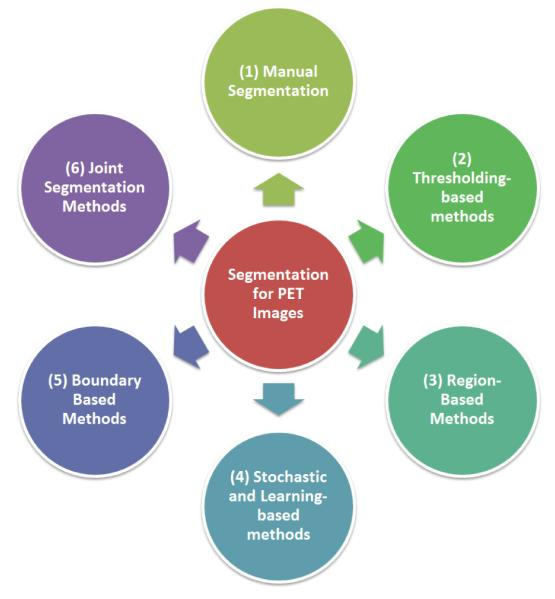
\includegraphics[scale=0.8]{cluster.jpg}
    \end{figure}
\end{frame}

%\subsection{Ручная сегментация}
%\begin{frame}
 %   \frametitle{Ручная сегментация}
  %  \begin{itemize}
   %     \item Конструирование размеченного множества изображений (ground truth)
    %    \item Оценка качества 
     %  \[DSC(V_1, V_2) = 2\frac{|V_1\cup V_2|}{|V_1|+|V_2|}\]
      % \item Сложности         
    %\end{itemize}
%\end{frame}

\subsection{Пороговые методы}
\begin{frame}
    \frametitle{Пороговые методы}
    \begin{itemize}
        \item Простой, интуитивно понятный и популярный метод,
        при котором черно-белое изображение конвертируется в бинарное, и пиксели больше определенного 
        значения считаются передним планом, а меньше - фоном.
        \item Сложность - определить оптимальное пороговое значение.        
    \end{itemize}
\end{frame}
\subsection{Стохастические модели и модели, основанные на обучении}
\begin{frame}
    \frametitle{Стохастические модели и модели, основанные на обучении}
    \begin{itemize}
        \item \textit{Mixture models} - объекты на ПЭТ-изображении
        имеют примерно гауссовское распределение и это априорное знание 
        может помочь в сегментации.
        \item \textit{Fuzzy locally adaptive Bayesian (FLAB) method} - статистический
        unsupervised метод, при котором считается, что изображение содержит два класса твердых
        тканей и конечное число \grqq нечетких уровней\glqq, которые 
        включают в себя смесь двух классов. Из-за свойства нечеткости 
        воксели принадлежат одному из двух классов, а уровень их 
        \grqq нечеткости\glqq определяется степенью принадлежности к каждому из классов.
        \item \textit{Clustering/Classification of PET image intensities}
        \begin{itemize}
            \item Классификация - разделение пространства объектов, полученного из изображения, с помощью известных меток
            \item Кластеризация - используется пространственная информацию, содержащаяся в изображениях, но без использования обучающих данных
        \end{itemize}
    \end{itemize}
\end{frame}

\subsection{Методы сегментации, основанные на регионах}
\begin{frame}
    \frametitle{Методы сегментации, основанные на регионах}
    Сегментация на основе регионов, в которых однородность 
    изображения является основным фактором для определения 
    границ объекта.
    \begin{itemize}
        \item \textit{Region Growing} - метод, который включает пространственную информацию в изображение наряду с информацией об интенсивности.
        \item \text{Графовые методы}
        \begin{itemize}
            \item Graph-cut
            \item Random walk

        \end{itemize}
        
    \end{itemize}
    
\end{frame}
\subsection{Методы выделения границ}
\begin{frame}
    \frametitle{Методы выделения границ}
    \begin{itemize}
        \item \textit{Active Contours (snakes)} - начальный контур 
        вокруг интересующего объекта деформируется и движется к желаемым границам.
        \item \textit{Level Set} - способ моделирования активных контуров путем отслеживания 
        границ между различными фазами потоков жидкости.
        \item \textit{Градиентные методы} - обычно, на границе происходит резкое изменение значения интенсивности. 
        Чтобы определить, где это происходит, вычисляется градиент между рассматриваемым вокселем и его соседями.
    \end{itemize}
\end{frame}

\subsection{Совместная сегментация}
\begin{frame}
    \frametitle{Совместная сегментация}
    \begin{itemize}
        \item Для сегментации совмещаются несколько изображений различных модальностей, 
        содержащих дополнительную информацию из входных данных. Обычно это ПЭТ/КТ и ПЭТ/МРТ.
    \end{itemize}
\end{frame}

\begin{frame}
    \frametitle{Метрики качества}
    \begin{itemize}
        \item Обучающая выборка: \(X^m=\{(x_1,y_1),\dots ,(x_m, y_m)\}\)
        \item Задача классификации на 2 класса: \(X\rightarrow Y, Y=\{+1, -1\}\)
        \item Алгоритм классификации \(a(x): X\rightarrow Y\)
        \item Доля ложных положительных классификаций
        \[FPR(a, X^m) = \frac{\sum_{i=1}^{m}[y_i=-1][a(x_i)=+1]}{\sum_{i=1}^{m}[y_i=-1]}=\frac{FP}{\sum_{i=1}^{m}[y_i=-1]}\]
        \item Доля верных положительных классификаций
        \[TPR(a, X^m) = \frac{\sum_{i=1}^{m}[y_i=+1][a(x_i)=+1]}{\sum_{i=1}^{m}[y_i=+1]}=\frac{TP}{\sum_{i=1}^{m}[y_i=+1]}\]
    \end{itemize}
\end{frame}

\begin{frame}
    \frametitle{Кривая ошибок}
    \begin{itemize}
        \item \textbf{ROC-кривая} - компромисс между уровнем ложной тревоги и долей 
        верного отклика 
    \end{itemize}
    \begin{figure}
        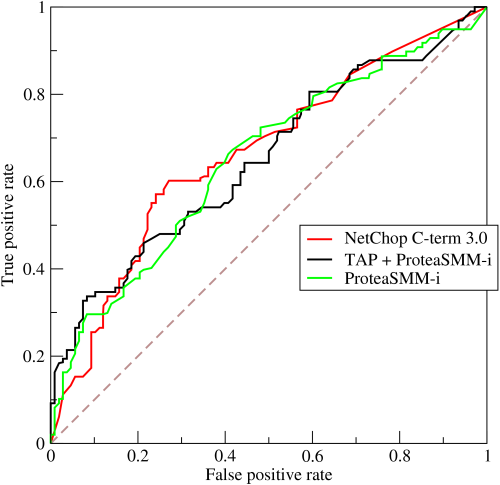
\includegraphics{roc_curve.png}
        \caption{По оси Х откладывается FPR, по оси Y - TPR}
    \end{figure}
\end{frame}
\begin{frame}
    \frametitle{Площадь под ROC-кривой}
    \begin{itemize}
        \item Чем больше для каждого значения ошибки FPR значение правильного 
        предсказания TPR, тем лучше работает классификатор. Т.о., площадь
        под кривой (Area Under Curve, AUC/AUROC) необходимо максимизировать.
    \end{itemize}
    \begin{figure}
        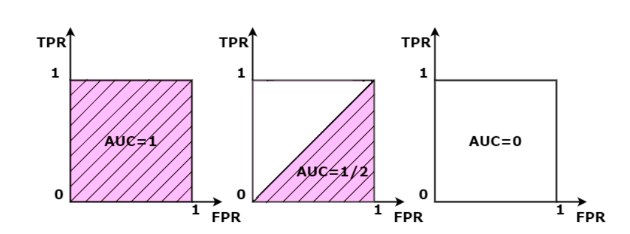
\includegraphics[scale=0.5]{auroc.png}
        \caption{ROC- кривые для наилучшего (AUC=1), случайного (AUC=0.5) 
        и наихудшего (AUC=0) алгоритма.}
    \end{figure}
\end{frame}